\documentclass[11pt,a4paper]{article}

%---- defitions ----
\def\Author{
\bf https://github.com/HIPERFIT/HQL
}
\def\Title{\bf Hiperfit Quant Library \\ Documentation}

\usepackage{tikz}
\usepackage{gnuplottex}
\usepackage[]{amsmath}
\usepackage{amssymb}
\usepackage[english]{babel}
\usepackage[utf8]{inputenc}
\usepackage{graphicx}
\usepackage{moreverb}
\usepackage{hyperref}
\usepackage{color}
\usepackage{listings,setspace,framed}
\usepackage{pgfplots}
%\usepackage{bashful}
\usepackage{tikz}
\usetikzlibrary{decorations.pathreplacing}
\usepackage{lmodern,inconsolata}
\usepackage{array, xcolor, lipsum, bibentry, fancyhdr}
\usepackage[absolute]{textpos}
\usepackage[top=25mm, bottom=25mm, left=22mm, right=22mm]{geometry} %Layout of page
\usepackage{lastpage} % number of last page 

%\usepackage[table]{xcolor}
%\usepackage[table]{xcolor}
%\usepackage{xcolor}
%\usepackage{filter}
%\usepackage{vim}
\usepackage{caption}
\usepackage[compatibility=true]{caption} 
\usepackage{etex}
\usepackage{ctable}
\captionsetup[figure]{labelfont=bf}
\captionsetup[table]{labelfont=bf,position=below}

\numberwithin{equation}{section}

%---- settings ----
% Comments
\newcommand{\comm}[2]{{\sf \(\spadesuit\){\bf #1: }{\rm \sf #2}\(\spadesuit\)}}
\newcommand{\mcomm}[2]{\marginpar{\scriptsize \comm{#1}{#2}}}
\newcommand{\ab}[1]{\mcomm{AB}{#1}}
\newcommand{\ja}[1]{\mcomm{JA}{#1}}

%\pagestyle{fancy}

\renewcommand{\headrulewidth}{0.5pt}
\renewcommand{\footrulewidth}{1pt}

%% Font size of tables
%\let\oldtabular\tabular
%\renewcommand{\tabular}{\small\oldtabular}

\usepackage[T1]{fontenc} % font
\setlength{\parindent}{0in}
\definecolor{lightgray}{rgb}{0.9,0.9,0.9}

\newenvironment{filecode}[1][]
{\minipage{\linewidth}
\lstset{basicstyle=\ttfamily\footnotesize,frame=single,
numberstyle=\small\color{black},keywordstyle=\color{black},commentstyle=\color{black},
stringstyle=\color{black},tabsize=2,backgroundcolor=\color{lightgray},language=Haskell,#1}}
{\endminipage}
\renewcommand*\rmdefault{ppl}

\lfoot{
\begin{textblock*}{100mm}(30mm, 280mm )
\end{textblock*}
}

\pagestyle{fancy}
\fancyhf{} 
 
\lhead{\uppercase{Hiperfit Quant Library}}
\rhead{\nouppercase{\rightmark}}
 
\cfoot{\thepage\ / \phantomsection\pageref*{LastPage}}
 
\lfoot{
\begin{textblock*}{100mm}(30mm, 280mm )
\end{textblock*}
}

%\newcolumntype{C}{>{\small}c}

%-------------------

\newcommand{\tikzmark}[1]{\tikz[overlay,remember picture] \node (#1) {};}
\newcommand{\DrawBox}[1][]{%
    \tikz[overlay,remember picture]{
    \draw[red,#1]
      ($(left)+(-0.2em,0.9em)$) rectangle
      ($(right)+(0.2em,-0.3em)$);}
}

\definecolor{comments}{rgb}{0,0.6,0}
\definecolor{strings}{rgb}{0.9,0,0}
\definecolor{keywords}{rgb}{0,0,0}
\definecolor{identifier}{rgb}{0.10,0.10,0.10}
\definecolor{background}{rgb}{0.98,0.98,0.98}


\lstdefinestyle{BashInputStyle}{
  language=haskell,
  breaklines=true,
  breakatwhitespace=true,
  frame=tblr,
  columns=fullflexible,
  backgroundcolor=\color{background},
  linewidth=1.0\linewidth,
  xleftmargin=0.1\linewidth,
  keywordstyle= \color{keywords},
  identifierstyle=\color{identifier},
  stringstyle=\color{strings},
  commentstyle=\color{comments},
  basicstyle=\fontsize{10}{12}\color{black}\ttfamily    
}

\lstdefinestyle{Output}{
  language=haskell,
  breaklines=true,
  breakatwhitespace=true,
  frame=tblr,
  columns=fullflexible,
  backgroundcolor=\color{gray!10},
  linewidth=1.0\linewidth,
  xleftmargin=0.1\linewidth,
  keywordstyle= \color{keywords}\bfseries,
  identifierstyle=\color{identifier},
  stringstyle=\color{strings},
  commentstyle=\color{comments},
  basicstyle=\fontsize{10}{12}\color{black}\bfseries
}

\lstset{escapechar=@,style=BashInputStyle}

\begin{document}

\title{HQL Documentation}

\title{\Title}
\author{\Author}
\date{\today}
\maketitle

\tableofcontents

\vskip 0.5\FrameSep

\section{Introduction}
This is the documentation of the Hiperfit Quant Library, HQL. As a reader you will
find valuable information about the theory behind the implementation together with
illustrative examples of real world use cases. The documentation itself is \textit{Literate Haskell}\cite{LitHaskell},
which means you can load this file into GHCi:

\vskip 0.5\FrameSep
\begin{lstlisting}
~/HQL$ ghci docs/hql.lhs
\end{lstlisting}

\section{Terminology}
In this section you'll find a the most commonly used words in this document, which are specific to the domain of finance and fixed income valuation.

\ctable[
caption = Terminology,
pos = ht,
doinside=\small
]{ll}{
}{
  \toprule
    Input & Meaning \\
  \midrule
    Settlement & Settlement date \\
    Maturity & Maturity date \\
    Period & Coupon payment period \\ 
    Basis & Day-count basis \\ 
    EndMonthRule & End-of-month payment rule \\ 
    IssueDate & Bond issue date \\ 
	Term & - \\
	Tenor & - \\
	LIBOR & - \\
	Annuity & - \\
	Bond & - \\
	Compounding & - \\
	Actual rate & - \\
	Annualized rate & - \\
  \bottomrule
}

\section{Compounding}
Compounding refers to the method where money accumulates during the progess of time. The oppostite of compounding is discounting.
When one talks about compounding, the interest rate or rate determines the rate at which the deposited amount of money will increase as a function of time.
Compounding is often separated into discrete and continous compounding.

\subsubsection{Discrete compounding}
Discrete compounding refers to compounding with fixed and known intervals of compounding, typically annually, semi-annually or quartlery.

\subsubsection{Linear discrete compounding}
$FV$, the future value in $T$ periods of a nominal $N$, is expressed as:

\[
FV_T = N(1+R_TT)
\]

where $R_T$ is the interest rate.

\subsubsection{Exponential discrete compounding}

Future value of a nominal cash flow $N$ under exponential compounding over
$n$ periods:

\[ FV_T = N(1+R_T)^n \]

The present value of a nominal future cash flow $N$ is therefore

\[ PV_T = \frac{N}{(1+R_T)^n} \]

Periodic compounding where $n$ is the number of times interest compounded per period

\[ 
FV_T=N\left( 1 + \frac{R}{n}  \right)^{nT}
\]

\subsection{Continuous compounding}
Continuous compounding is defined as taking the limit of the discrete compounding as n goes to infinity,
\[ 
FV=\lim_{n \to \infty} N \left(1+\frac{R}{n}\right)^{nT}=Ne^{RT}
\]

%\begin{minipage}{\linewidth}
%\begin{figure}[h]
%\centering
%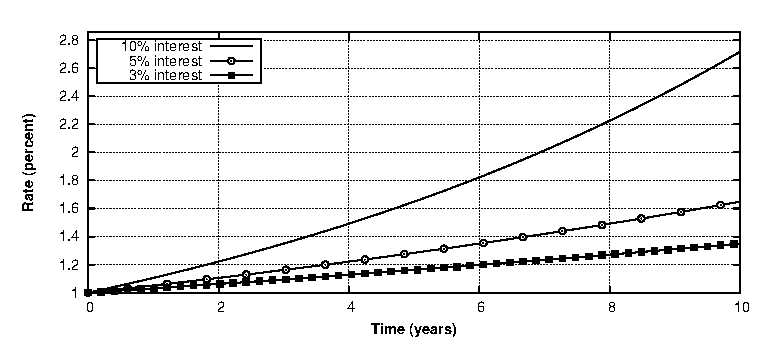
\includegraphics[scale=.50]{gnuplot/comp01.eps}
%\caption{Continuous compounding with various rates}
%\label{fig:digraph}
%\end{figure}
%\end{minipage}

\begin{minipage}{\linewidth}
\makebox[\linewidth]{%
  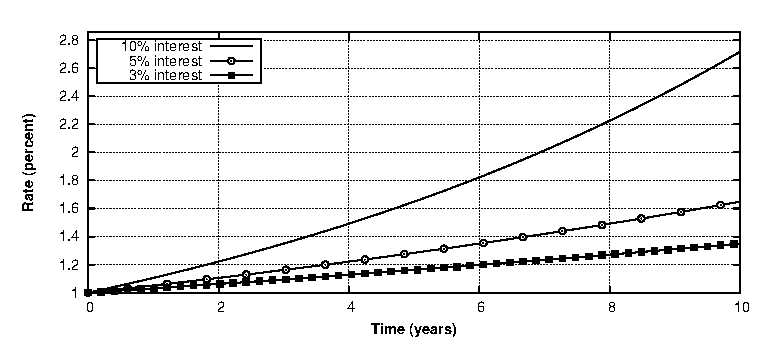
\includegraphics[keepaspectratio=true,scale=1.0]{gnuplot/comp01.eps}}
\captionof{figure}{Continuous compounding with various rates}
\label{visina8}
\end{minipage}

\subsection{Transition between discrete and continuous}
Table of interest rates at various compounding frequencies.

\ab{Jost said we need to describe the table here}

The table below illustrates the effect of compounding at various frequencies. The nominal rate
is the annualized interest rate, compounded once per year. As the frequency increases, the discrete
rate almost equals the continous one.

\ctable[
caption = Interest rates at various compounding frequencies,
pos = ht,
doinside=\small
]{lllllll}{
}{
\toprule
 Nominal Rate &  Semi-Annual & Quarterly &  Monthly &  Weekly &  Daily  & Continuous \\
  \midrule
    1.0000       & 1.0025       & 1.0038     & 1.0046   & 1.0049  & 1.0050  & 1.0050      \\
    2.0000       & 2.0100       & 2.0151     & 2.0184   & 2.0197  & 2.0201  & 2.0201      \\
    5.0000       & 5.0625       & 5.0945     & 5.1162   & 5.1246  & 5.1267  & 5.1271      \\
    10.0000      & 10.2500      & 10.3813    & 10.4713  & 10.5065 & 10.5156 & 10.5171     \\
    15.0000      & 15.5625      & 15.8650    & 16.0755  & 16.1583 & 16.1798 & 16.1834     \\
    20.0000      & 21.0000      & 21.5506    & 21.9391  & 22.0934 & 22.1336 & 22.1403     \\
    25.0000      & 26.5625      & 27.4429    & 28.0732  & 28.3256 & 28.3916 & 28.4025     \\
    50.0000      & 56.2500      & 60.1807    & 63.2094  & 64.4788 & 64.8157 & 64.8721     \\ 
  \bottomrule
}

\subsection{Calculating present and future value}
%To calculate the present value of a future cash flow we use the discount factor
%to scale the amount:

%We can calculate the future value by using the inverse of the discount factor above:

To calculate present and future value in HQL, two objects are of particular interest:
the DiscountFactor and the CompoundFactor. Let's start by using the DiscountFactor in an example
where we have a monthly compounded interest rate of 8.5\% during a period of 3 years:
\vskip 0.5\FrameSep
\begin{lstlisting}
HQL> let df = discountFactor (InterestRate (Periodic 12) 8.5) 3.0 0.0
\end{lstlisting}
We can use the previously defined DiscountFactor to discount an arbitrary amount. Let's say
\$1000.00:
\vskip 0.5\FrameSep
\begin{lstlisting}
HQL> df*1000.0
\end{lstlisting}
yields the following output:
\vskip 0.5\FrameSep
\begin{lstlisting}[style=Output]
775.6133702070988
\end{lstlisting}

\subsection{The continuous discount factor}
The \textit{continuous discount factor} with maturity $T$ at time $t$ is defined as,
\[
p(t,T)=e^{-r(T-t)}; T>t
\]
Which equals the \textit{zero-coupon unit bond}, with face $N=1$. The discount factor
can be seen as entities in a vector, the \textit{discount function},

\[
\mathbf{df} = (p(t,T_1), ..., p(t,T_n))
\]

In the same way, cash flows can be considered entities in a vector,

\[
\mathbf{cf} = (c_1, ..., c_i)
\]

For example, if we were to calculate the present value of a series of future cash flows,
\[
\mathbf{cf} = (\$1000.00,\$1500.00,\$1000.00,\$2000.00)
\]
We can multiply by the discount function with $T_n=n$ years and the rate at 5.00\% continuously compounded,
\[
p(0) = \mathbf{df}\cdot\mathbf{cf} = (e^{-rT_1},...,e^{-rT_n})\cdot(p(0,T_1), ...,p(0,T_4))=
\]
\[
(e^{-0.05\cdot1},e^{-0.05\cdot2},e^{-0.05\cdot3},e^{-0.05\cdot4}) \cdot (\$1000.00,\$1500.00,\$1000.00,\$2000.00)=
\]
\[
(\$951.23,\$1357.26,\$860.71,\$1637.46)
\]

The above calculation is done in HQL using the function \textit{zipWith} taking the discount function and the list of future cash flows as arguments.
\vskip 0.5\FrameSep
\begin{lstlisting}
HQL> zipWith (*) (discountFactors (interestRate Continuous 5.0) 5 4 <*> pure 0) [1000,1500,1000,2000]
\end{lstlisting}
\vskip 0.5\FrameSep
yields the following output:
\vskip 0.5\FrameSep
\begin{lstlisting}[style=Output]
[951.229424500714,1357.2561270539393,860.7079764250578,1637.4615061559637]
\end{lstlisting}
\vskip 0.5\FrameSep
A slightly modified version will return the sum of the cash flows. This is the basis of bond pricing, which is covered in section \nameref{sec:fi}.
\vskip 0.5\FrameSep
\begin{lstlisting}
HQL> sum $ zipWith (*) (discountFactors (interestRate Continuous 5.0) 5 4 <*> pure 0) [1000,1500,1000,2000]
\end{lstlisting}
\vskip 0.5\FrameSep
yields the following output:
\vskip 0.5\FrameSep
\begin{lstlisting}[style=Output]
4806.655034135675
\end{lstlisting}


\section{Interest rates}

- annualized rate (nominal rate)
- actual rate

\ctable[
caption = The caption is centered by default,
pos = h,
doinside=\small,
center,
]{llll}{
}{
\toprule
    Maturity (months) & Spot rate & Forward & Rate \\
  \midrule
    3 & 4.5\% & $F_{0,3}$ & 4.5\% \\
    6 & 4.3\% & $F_{3,3}$ & 4.05\% \\
    9 & 4.2\% & $F_{6,3}$ & 3.92\% \\
    12 & 4.0\% & $F_{9,3}$ & 3.3\% \\
  \bottomrule
}

\subsection{Spot rates}
Spot rates refers to rates that are observable at present time in the market.
Spot rates are quoted on an annualized basis.

\subsection{Forward rates}
Forward rates indicate the interest rate between two future dates [S,T]
\[
(1+R_T)^T=(1+R_S)^S(1+R(t;S,T))^{T-S}; T>S
\]
Solving for the forward rate yields
\[
R(t=0,S,T)=\left( \frac{(1+R_T)^T}{(1+R_S)^S} - 1 \right)^{\frac{1}{T-S}};T>S
\]

Continuous compounding version of the above

\[
e^{R_TT}=e^{R_SS}e^{R(t;S,T)(T-S)};T>S
\]
Solving for the forward rate
\[
R(t;S,T)=\frac{R_TT-R_SS}{T-S}
\]

Let's look at an example of how to determine the forward rate given two time periods and interest rates. The input parameters are listed in the table below.

\ctable[
caption = Input parameters to example,
pos = ht,
width=80mm,
center,
doinside=\small
]{ll}{
}{
  \toprule
    Parameter & Value \\ 
  \midrule
    Compounding & Semi-annually ($n=2$)\\
    $\tau_1$ & 0.25\\
    $\tau_2$ & 1.5 \\
    $R_1$ & 6.65 \\
    $R_2$ & 7.77 \\
  \bottomrule
}

\vskip 0.5\FrameSep
\begin{lstlisting}
HQL> (((discountFactor (InterestRate (Periodic 2) 6.65) 0.25 0.0)/(discountFactor (InterestRate (Periodic 2) 7.77) 1.5))**(1/(2*1.25))-1)*2*100
\end{lstlisting}
yields the following output:
\vskip 0.5\FrameSep
\begin{lstlisting}[style=Output]
7.994727369824384
\end{lstlisting}

\subsection{LIBOR}
The LIBOR (London InterBank Offered Rate) interest rate is the most important interbank rate
used for fixed income valuation. LIBOR rates are quoted on a simple compounding basis with maturities
from overnight to 12 months.

The rate quoted is the annualized rate, to calculate the actual rate we do as follows...

LIBOR comes in 8 maturities
5 different currencies
\\
\\
Table of LIBOR rates per 2013-12-26,

\ctable[
caption = LIBOR rates 2013-12-26,
pos = ht,
width=60mm,
center,
doinside=\small
]{ll}{
}{
  \toprule
    Period & LIBOR \\
  \midrule
    1 month & 0.17\% \\ 
    3 month & 0.24\% \\
    6 month & 0.35\% \\
    12 month & 0.59\% \\
  \bottomrule
}


%$R$ is the annual rate
%The value after m compounding periods with n compounding periods per year

\[ 
1+(T-S)L=\frac{p(t,S)}{p(t,T)}
\]
\[ 
e^{r(T-S)}=\frac{p(t,S)}{p(t,T)}
\]
\\
\textbf{LIBOR forward rate}
Simply-compounded forward rate $[S,T]$ prevailing at time $t$,
\[
L(S,T) = -\frac{p(S,T)-p(t,S)}{(T-S)p(t,T)}
\]
\\
\textbf{LIBOR spot rate},

\[
L(S,T)=\frac{p(S,T)-1}{(T-S)p(S,T)}
\]
\\
\textbf{LIBOR forward rate},
Continuously compounded forward rate $[S,T]$ prevailing at time $t$,

\[
R(t;S,T)=-\frac{\log{p(t,T)}-\log{p(t,S)}}{T-S}
\]
\\
\textbf{LIBOR spot rate},
\[
R(S,T)=\frac{\log{p(S,T)}}{T-S}
\]
\\
\textbf{Instantaneous forward rate},
\[
f(t,T)=-\frac{\partial\log{p(t,T)}}{\partial{T}}
\]
\\
\textbf{Instantaneous short rate},
\[
r(t)=f(t,t)
\]

For example, the three-month forward LIBOR for the period $[S,T]$, where $T=S+\tau$ and $\tau=1/4$,
\[
L(t,T) = F(t;S,S+\tau) = F(t;S,T), T>S
\]

\subsubsection{Calculating LIBOR rates}

\section{Interest rate Swaps}
\subsection{Theory and valuation}
\subsection{Cash flows}
\section{Bonds}
\label{sec:fi}

\subsection{Zero coupon bond}
Zero coupon bond and the discount factor

\subsection{Fixed coupon bond}
Series of payments called coupons and a nominal value N (face value)
A number of future payment dates $T_1 < ... < T_n$ where is the maturity of the bond
A sequence of deterministic coupons $c_1, ..., c_n$

\[ c_{T_i} = \left\{
\begin{array}{ll}
  Nc, & \text{for } i=1,...,n-1,  \\
  N(c+1), &\text{for } i=n.
\end{array} \right.\]

\[
p(t) = N \cdot p(t,T_n)+\sum_{i=1}^{n} (c_ip(t,T_i))
\]
From above, we can see that the fixed coupon bond can be reconstructed by a portfolio of zero
bonds (scaled by the coupon), $p(t,T)$ is a zero bond with N=1.
\[
p(t)=\left[p(t,T_n)+r\delta\sum_{i=1}^{n} p(t,T_i)\right]\cdot N
\]
Where $r$ is the coupon rate. For a standardized coupon bond the time intervals will be equally
spaced according to
\[
T_i=T_0+i\delta
\]

Convert above to a list of payments at offset times. Where denotes the time interval in years
according to the day-count convention, see below.

\subsubsection{Example - Calculating present value}

\ctable[
caption = Input parameters to example,
pos = h,
center,
doinside=\small
]{llllll}{
}{
  \toprule
    Maturity (years) & 1 & 2 & 3 & 4 & 5\\ 
  \midrule
    Interest rate & 3.00\% & 3.25\% & 3.50\% & 3.55\% & 3.30\%\\
  \bottomrule
}

Let's consider a bond maturing in 5 years, paying a coupon of 10\% and a face of 1000,
\ctable[
caption = Bond price,
pos = h,
center,
doinside=\small
]{lllll}{
}{
  \toprule
    Maturity & Interest rate & Cash flow & Present value \\
  \midrule
    1 & 3.00\% & 100 & 97.09 \\
    2 & 3.25\% & 100 & 93.80 \\
    3 & 3.50\% & 100 & 90.19 \\
    4 & 3.55\% & 100 & 86.98 \\
    5 & 3.30\% & 1100 & 935.17 \\
\midrule
    Price bond  &     &  & \textbf{1303.23} \\
  \bottomrule
}

\framebox{TODO: Adapt HQL to handle this case}

\subsection{Floating coupon bond}
Not yet supported by HQL (this means stochastic interest rates).

\section{Standard bond types}

We now present the bonds supported in HQL.

\subsection{Annuity}

An annuity is an example of an amortized bond meaning that the debitor repays the
face value over its lifetime. Payments are distributed equally over all the settlement
dates, increasing and decreasing the repayment amount and coupon respectively (see figure
\ref{fig:annuitycf}.

\begin{figure}[h!]
\begin{center}
\begin{tikzpicture}[-,shorten >=1pt,auto,node distance=1.5cm,thick,minimum size=0.8cm,main node/.style={circle,draw=red,very thick}]
\tikzstyle{selected edge} = [draw,line width=6pt,-,blue!30]

\coordinate (belowstart) at (0,-1);
\coordinate (start) at (0,0);
\coordinate (stop) at (10.2,0);
\coordinate (abovestop) at (10.2,2);
\draw (start) -- (stop);
\draw (start) -- (belowstart);
\draw (stop) -- (abovestop);

\node at (0, -1.5) () {$t=0$};

\filldraw[draw=black, fill=blue] (2,0) rectangle node {} +(0.2,1.5);
\filldraw[draw=black, fill=red]  (2,1.5) rectangle node {} +(0.2,0.25);
\node at (2, 2.5) () {$t=2$};

\filldraw[draw=black, fill=blue] (4,0) rectangle node {} +(0.2,1.3);
\filldraw[draw=black, fill=red]  (4,1.3) rectangle node {} +(0.2,0.45);
\node at (4, 2.5) () {$t=4$};

\filldraw[draw=black, fill=blue] (6,0) rectangle node {} +(0.2,1.1);
\filldraw[draw=black, fill=red]  (6,1.1) rectangle node {} +(0.2,0.65);
\node at (6, 2.5) () {$t=6$};

\filldraw[draw=black, fill=blue] (8,0) rectangle node {} +(0.2,1);
\filldraw[draw=black, fill=red]  (8,1) rectangle node {} +(0.2,0.75);
\node at (8, 2.5) () {$t=8$};

\filldraw[draw=black, fill=blue] (10,0) rectangle node {} +(0.2,0.85);
\filldraw[draw=black, fill=red]  (10,0.85) rectangle node {} +(0.2,0.9);
\node at (10, 2.5) () {$t=10$};

% Legend
\filldraw[draw=black, fill=blue] (7,-1) rectangle node {} +(0.2,0.2);
\node at (8.3, -0.92) () {repayment};

\filldraw[draw=black, fill=red] (7,-1.5) rectangle node {} +(0.2,0.2);
\node at (8, -1.44) () {coupon};

\end{tikzpicture}
\caption{Cashflow of an annuity.}
\label{fig:annuitycf}
\end{center}
\end{figure}

\subsubsection{Example}
Suppose we want to price an annuity maturing in 5 years, a face of \$1000.00 at an annual interest rate of 5.00\%.
This can be done in continuous time integrating the continuous discount factor $e^-rt$:
\[
p(0)=N\cdot \int_{t=0}^T \mathrm{e}^{-rt}\,\mathrm{d}t=\frac{N}{R}\cdot (e^{-rt}-e^{-rT})=\frac{N}{R}(1-e^{-rT})
\]
Plugging in the numbers from above gives:
\[
p(0)=\frac{\$1000.00}{0.05}(1-e^{-\log(1+0.005)\cdot 5})\approx \$4329.48
\]
\begin{lstlisting}
HQL> df*1000.0
\end{lstlisting}
yields the following output:
\vskip 0.5\FrameSep
\begin{lstlisting}[style=Output]
775.6133702070988
\end{lstlisting}

\subsection{Bullet}

Bullet has a fixed rate coupon which is paid at every settlement. No repayments before maturity. Figure \ref{fig:bulletcf} shows the cashflows.

\[ p(t,T) = \sum_{t=1}^{T}\frac{C}{(1+r)^t} + \frac{N}{(1+r)^T} \]

\begin{figure}[h!]
\begin{center}
\begin{tikzpicture}[-,shorten >=1pt,auto,node distance=1.5cm,thick,minimum size=0.8cm,main node/.style={circle,draw=red,very thick}]
\tikzstyle{selected edge} = [draw,line width=6pt,-,blue!30]

\coordinate (belowstart) at (0,-1);
\coordinate (start) at (0,0);
\coordinate (stop) at (10.2,0);
\coordinate (abovestop) at (10.2,2);
\draw (start) -- (stop);
\draw (start) -- (belowstart);
\draw (stop) -- (abovestop);

\node at (0, -1.5) () {$t=0$};

\filldraw[draw=black, fill=red]  (2,0) rectangle node {} +(0.2,0.25);
\node at (2, 2.5) () {$t=2$};

\filldraw[draw=black, fill=red]  (4,0) rectangle node {} +(0.2,0.25);
\node at (4, 2.5) () {$t=4$};

\filldraw[draw=black, fill=red]  (6,0) rectangle node {} +(0.2,0.25);
\node at (6, 2.5) () {$t=6$};

\filldraw[draw=black, fill=red]  (8,0) rectangle node {} +(0.2,0.25);
\node at (8, 2.5) () {$t=8$};

\filldraw[draw=black, fill=blue] (10,0) rectangle node {} +(0.2,1);
\filldraw[draw=black, fill=red]  (10,1) rectangle node {} +(0.2,0.25);
\node at (10, 2.5) () {$t=10$};

% Legend
\filldraw[draw=black, fill=blue] (7,-1) rectangle node {} +(0.2,0.2);
\node at (8.3, -0.92) () {repayment};

\filldraw[draw=black, fill=red] (7,-1.5) rectangle node {} +(0.2,0.2);
\node at (8, -1.44) () {coupon};

\end{tikzpicture}
\caption{Cashflow of a bullet.}
\label{fig:bulletcf}
\end{center}
\end{figure}


\subsection{Consol}
Consol has a fixed rate coupon and never terminates and there is no payments at any
settlement, only interest (the coupon) is paid. Figure \ref{fig:consolcf} shows this
pictorially.

\[
p(t) = N \cdot p(t,T_n)+\sum_{i=1}^{n} (c_i \cdot p(t,T_i))
\]
\[
\lim_{x \to \infty} p(t,\infty)=\left[r\delta\sum_{i=1}^{\infty} p(t,T_i)\right]\cdot N = 
\sum_{i=0}^{\infty} p(t,T_i) \cdot \frac{\delta N}{e^{rT}} \cdot \to \frac{\delta N}{e^{rT}}\left[ \frac{e^{rT}}{r}\right] = \frac{\delta N}{r}
\]
Which means the present value of the consol bond is represented by the the following formula:
\[
p(t) = \frac{\delta N}{r}
\]

\framebox{p(t) function of time?}

\begin{figure}[h!]
\begin{center}
\begin{tikzpicture}[-,shorten >=1pt,auto,node distance=1.5cm,thick,minimum size=0.8cm,main node/.style={circle,draw=red,very thick}]
\tikzstyle{selected edge} = [draw,line width=6pt,-,blue!30]

\coordinate (belowstart) at (0,-1);
\coordinate (start) at (0,0);
\coordinate (stop) at (9.2,0);
\coordinate (dotstop) at (10.2,0);
\draw (start) -- (stop);
\draw (start) -- (belowstart);
\draw[dotted] (stop) -- (dotstop);

\node at (0, -1.5) () {$t=0$};

\filldraw[draw=black, fill=red]  (2,0) rectangle node {} +(0.2,0.25);
\node at (2, 2.5) () {$t=2$};

\filldraw[draw=black, fill=red]  (4,0) rectangle node {} +(0.2,0.25);
\node at (4, 2.5) () {$t=4$};

\filldraw[draw=black, fill=red]  (6,0) rectangle node {} +(0.2,0.25);
\node at (6, 2.5) () {$t=6$};

\filldraw[draw=black, fill=red]  (8,0) rectangle node {} +(0.2,0.25);
\node at (8, 2.5) () {$t=8$};

% Legend
\filldraw[draw=black, fill=red] (7,-1) rectangle node {} +(0.2,0.2);
\node at (8.3, -0.92) () {coupon};

\end{tikzpicture}
\caption{Cashflow of a consol.}
\label{fig:consolcf}
\end{center}
\end{figure}

\subsection{Serial}

Serial is an amortized bond with a fixed rate coupon, the repayments are spread evenly over all remaining settlements and the coupon payments, $C_t$ decline over time as depicted in figure
\ref{fig:serialcf}.

\[ p(t,T) = \sum_{t=1}^{T}\frac{C_t}{(1+r)^t} + \frac{N}{(1+r)^T} \]

\begin{figure}[h!]
\begin{center}
\begin{tikzpicture}[-,shorten >=1pt,auto,node distance=1.5cm,thick,minimum size=0.8cm,main node/.style={circle,draw=red,very thick}]
\tikzstyle{selected edge} = [draw,line width=6pt,-,blue!30]

\coordinate (belowstart) at (0,-1);
\coordinate (start) at (0,0);
\coordinate (stop) at (10.2,0);
\coordinate (abovestop) at (10.2,2);
\draw (start) -- (stop);
\draw (start) -- (belowstart);
\draw (stop) -- (abovestop);

\node at (0, -1.5) () {$t=0$};

\filldraw[draw=black, fill=blue] (2,0) rectangle node {} +(0.2,1);
\filldraw[draw=black, fill=red]  (2,1) rectangle node {} +(0.2,1);
\node at (2, 2.5) () {$t=2$};

\filldraw[draw=black, fill=blue] (4,0) rectangle node {} +(0.2,1);
\filldraw[draw=black, fill=red]  (4,1) rectangle node {} +(0.2,0.75);
\node at (4, 2.5) () {$t=4$};

\filldraw[draw=black, fill=blue] (6,0) rectangle node {} +(0.2,1);
\filldraw[draw=black, fill=red]  (6,1) rectangle node {} +(0.2,0.5);
\node at (6, 2.5) () {$t=6$};

\filldraw[draw=black, fill=blue] (8,0) rectangle node {} +(0.2,1);
\filldraw[draw=black, fill=red]  (8,1) rectangle node {} +(0.2,0.25);
\node at (8, 2.5) () {$t=8$};

\filldraw[draw=black, fill=blue] (10,0) rectangle node {} +(0.2,1);
\filldraw[draw=black, fill=red]  (10,1) rectangle node {} +(0.2,0.1);
\node at (10, 2.5) () {$t=10$};

% Legend
\filldraw[draw=black, fill=blue] (7,-1) rectangle node {} +(0.2,0.2);
\node at (8.3, -0.92) () {repayment};

\filldraw[draw=black, fill=red] (7,-1.5) rectangle node {} +(0.2,0.2);
\node at (8, -1.44) () {coupon};

\end{tikzpicture}
\caption{Cashflow of a serial.}
\label{fig:serialcf}
\end{center}
\end{figure}


\framebox{TODO: Continous time and HQL}

\section{US Treasury Bonds}
Treasury securities are the debt financing instruments of the United States federal government, and they are often referred to simply as Treasuries.
\subsection{Treasury Bill - T-Bill}
Short term debt instruments that mature in one year or less.
\subsection{Treasury Note - T-Note}
Medium term debt instruments that mature in two to ten years.
\subsection{Treasury Bond - T-Bond}
Long term debt instruments that mature in twenty to thirty years.

\subsection{Example using HQL}

\section{The term structure}

A \textbf{term structure of interest rates} refers to the general relation between yield and maturity that exists in a given bond market. If the term structure is derived from zero-coupon bonds it forms a good basis for pricing analysis of \emph{any} bond.\\

A \textbf{yield curve} is a plot of a specific set of bond yields as a function of their maturity. This is not good for general pricing or valuation purposes, except for the specific bonds plotted. The key difference between a term structure and a yield curve is that we discount \emph{any} cashflow by using former, while the latter is only applicable for bonds who's yields correspond. Figure SOMETHING 

The term structure or the yield curve.
Created from zero coupon bonds, zero yield curve
\[
y(t,T)=-\frac{\log{p(t,T)}}{T-t}
\]
The yield curve is constructed by fixating $t$,
\[
T\to y(t,T)
\]
To obtain the discount factor from a yield curve at time $t$,
\[
e^{y(t,T)(T-t)}=e^{-\log{p(t,T)}}\iff e^{y(t,T)(T-t)}=\frac{1}{p(t,T)}
\]
\[
\iff p(t,T)=e^{-y(t,T)(T-t)}
\]
We can price a bond from the yield curve, given face value $N$,
\[
p(t,T)=e^{-y(t,T)(T-t)}\cdot N
\]


\begin{figure}[h!]
\begin{center}
\begin{tikzpicture}[-,shorten >=1pt,auto,node distance=1.5cm,thick,minimum size=0.8cm,main node/.style={circle,draw=red,very thick}]
\tikzstyle{selected edge} = [draw,line width=6pt,-,blue!30]

\coordinate (belowstart) at (0,-1);
\coordinate (xaxis) at (10,0);
\coordinate (origo) at (0,0);
\coordinate (yaxis) at (0,5);

% Draw axes
\draw[->] (origo) -- (xaxis) node[right] {Time to maturity};
\draw[->] (origo) -- (yaxis) node[above] {Interest rate};

% Flat TS
\draw[thick,draw=blue] (0,1.5) -- (10,1.5);
% "Normal" TS
\draw[thick,draw=green] (0,0) parabola[bend at end] (10,5);
% Inverse TS
\draw[thick,draw=red] (0,5) parabola[bend at end] (10,0.5);

% Legend
\filldraw[draw=black, fill=blue] (5.2,-1) rectangle node {} +(0.2,0.2);
\node at (6, -0.92) () {Flat};

\filldraw[draw=black, fill=green] (0,-1) rectangle node {} +(0.2,0.2);
\node at (1.55, -0.92) () {Logarithmic};

\filldraw[draw=black, fill=red] (3,-1) rectangle node {} +(0.2,0.2);
\node at (4.15, -0.92) () {Inverted};

\end{tikzpicture}
\caption{An example of different term structures.}
\label{fig:anc}
\end{center}
\end{figure}


\subsection{Flat term structure}
\begin{lstlisting}
HQL> let termStructure x = 5 + (1/2)*sqrt(x)
HQL> discountFactor (InterestRate (Periodic 2) (termStructure 1.5)) 1.5 0.0
\end{lstlisting}

yields the following output:
\vskip 0.5\FrameSep

\begin{lstlisting}[style=Output]
0.9203271932613013
\end{lstlisting}

\subsection{Analytic term structure}

\subsection{Interpolated term structure}
Construct a term structure from bond prices, example

\subsubsection{Example - Treasury term structure}
In this example we are going to create a term structure form the data available for
US treasury bonds. Below is a table with data from 2013-12-26.

\ctable[
caption = US Treasury data 2013-12-26,
pos = ht,
width=80mm,
center,
doinside=\small
]{ll}{
}{
  \toprule
    Instrument & Yield \\
  \midrule
    3-month treasury bill & 0.07\% \\
    1-year treasury bill & 0.13\% \\
    2-year treasury note & 0.42\% \\
    5-year treasury note & 1.74\% \\
    10-year treasury note & 3\% \\
    30-year treasury bond & 3.92\% \\
  \bottomrule
}

\section{Yield curve fitting}
Various methods of fitting a yield curve to data (LIBOR, forex futures, bonds).

\begin{lstlisting}
HQL> df*1000.0
\end{lstlisting}
yields the following output:
\vskip 0.5\FrameSep
\begin{lstlisting}[style=Output]
775.6133702070988
\end{lstlisting}

\subsection{Yield to maturity}

The yield of a bond is the discount rate that makes the future value of all future
cashflows equal to the present value. For coupon payments $C_i$, bond price $N_t^T$
at time $t$ with maturity $T$, the yield $y_t$ satisfies: 

\[
N_t^T = \sum_{T_i > t} C_i (1+y_t)^{-(T_i - t)}, \hspace{2cm} \forall\; T_i < T
\]

For zero-coupon bonds, we therefore have the following for a maturity $T$ at
time $t$:

\[
N_t^T = (1+y_t^T)^{-(T-t)}
\]

with yield, $y_t^T$:

\[
y_t^T = \sqrt[T-t]{N_t^T} - 1
\]

\ab{Note on perpetual bonds}

\subsection{Duration and convexity}

\section{Day-count conventions}
Day-count convention or year fraction, time between two dates t and T.

\framebox{HQL example usage goes here}

\ctable[
caption = Input parameters to example,
pos = ht,
width = 80mm,
center,
doinside=\small
]{lll}{
}{
  \toprule
    Convention & Time interval & $\delta$ \\
  \midrule
    Actual/365 & Annually & 1.0 \\ 
    180/360 & Semi-annually & 0.5 \\ 
    90/360 & Quarterly & 0.25 \\ 
    30/360 & Monthly & 1/12 \\
  \bottomrule
}

Time is measured in years. Day-count conventions describe the time measurement between two
dates t and T. Dates are expressed by (day, month, year). 

\[ \tau = \boldsymbol{T} - \boldsymbol{t};  \left\{
  \begin{array}{l l}
      \boldsymbol{t} = (Y_1, M_1, D_1) \\
\boldsymbol{T}=(Y_2,M_2,D_2)
  \end{array} \right.\]


\subsection{Actual/365}
A year has 365 days, and the days are counted normally:
\[
\delta = \frac{\Delta \tau_D}{365} = \frac{D_2-D_1}{365} = \frac{\text{actual days between } \boldsymbol{t} \text{ and } \boldsymbol{T}}{365}
\]
\subsection{Actual/360}
Same as above except one year is said to be 360 days. Standard for US dollars
\[
\delta = \frac{\Delta \tau_D}{360} =\frac{D_2-D_1}{360} = \frac{\text{actual days between } \boldsymbol{t} \text{ and } \boldsymbol{T}}{360}
\]
\subsection{30/360}
Month are 30 days long, a year is 360 days long
\[
\delta = \frac{360 \cdot \Delta \tau_Y + 30 \cdot \Delta \tau_M + \Delta \tau_D}{360} =\frac{360(Y_2-Y_2)+30(M_2-M_1)+(D_2-D_1)}{360}
\]

\subsection{Business day conventions}
A business day convention is a convention for adjustment of dates when a specified date is not a good business day. 
\begin{description}
  \item[Following] \hfill \\
The adjusted date is the following good business day \ldots
  \item[Preceding] \hfill \\
    The adjusted date is the preceding good business day \ldots
  \item[Modified following] \hfill \\
  The adjusted date is the following good business day unless the day is in the next calendar month \ldots
  \item[End of month] \hfill \\
Where the start date of a period is on the final business day of a particular calendar month \ldots
\end{description}

\newpage

% REFERENCES
\bibliographystyle{abbrv}
%\addcontentsline{toc}{section}{References}
\bibliography{hql}

\end{document}
